\documentclass[xcolor=dvipsnames,aspectratio=169,t]{beamer}
  % t means frames are vertically centered to the top
\usepackage{slides-header}
\title{Eigenvalues and Eigenvectors}

\begin{document}
\maketitle

\begin{frame}{Introduction}
  \bigskip

  The concepts of \alert{eigenvalues} and \alert{eigenvectors} of a matrix are useful throughout pure and applied mathematics.
  \bi
  \ii Eigenvalues are used to study difference equations and continuous dynamical systems. 
  \ii They provide critical information in engineering design, and they arise naturally in such fields as physics and chemistry.
  \ei
\end{frame}

\begin{frame}{Introduction}
  \bigskip
  
  %TODO: I changed this 2x2 example so that the eigenvalues are smaller so that it works better on Desmos.  This is different than the 2x2 example that Adam had that shows up later.  It would be better to make a new example that could be used throughout for consistency, but that does not have the messy values, and that have small eigenvalues.
  
  Consider the linear transformation $T\colon\mathbb{R}^2\to\mathbb{R}^2$ where 
  $T(\mathbf{x})=A\mathbf{x}=\begin{bmatrix} 0 & -2 \\ -1 & 2 \end{bmatrix}\mathbf{x}$.
  \medskip
  
  How do $\mathbf{x}$ and $A\mathbf{x}$ relate?
  \bigskip
  
  \url{https://www.desmos.com/calculator/jovijh4fad}
  \vspace*{2em}

  \pause
  \begin{tasks}(2)
  \task Compute $A\u$, where $\u = \begin{bmatrix} 1+\sqrt{3} \\ 1 \end{bmatrix}$.
  \task Compute $A\v$, where $\v = \begin{bmatrix} -1 \\ 1 \end{bmatrix}$.
  \end{tasks}

  \begin{columns}[T]
  \column{0.6\tw}
  \colorb{\[  \begin{bmatrix} 0 & -2 \\ -1 & 2 \end{bmatrix}\begin{bmatrix} 1+\sqrt{3} \\ 1 \end{bmatrix} = \begin{bmatrix} -2 \\ 1-\sqrt{3} \end{bmatrix} = (1-\sqrt{3}) \mathbf{u} .\]}

  \column{0.4\tw}
  \alert{\[  \begin{bmatrix} 0 & -2 \\ -1 & 2 \end{bmatrix}\begin{bmatrix} -1 \\ 1 \end{bmatrix} = \begin{bmatrix} -2 \\ 3 \end{bmatrix} \ne c \mathbf{v} .\]}
  \end{columns}
\end{frame}


\begin{frame}{Eigenvalues and Eigenvectors}
  \bigskip

  Consider the matrix $A = \begin{bmatrix} 0 & -2 \\ -1 & 2 \end{bmatrix}$ and vectors $\u = \begin{bmatrix} 1+\sqrt{3} \\ 1 \end{bmatrix}$ and $\v = \begin{bmatrix} -1 \\ 1 \end{bmatrix}$.
  \medskip

  \begin{columns}[T]
  \column{0.6\tw}
  \colorb{\[  \begin{bmatrix} 0 & -2 \\ -1 & 2 \end{bmatrix}\begin{bmatrix} 1+\sqrt{3} \\ 1 \end{bmatrix} = \begin{bmatrix} -2 \\ 1-\sqrt{3} \end{bmatrix} = (1-\sqrt{3}) \u .\]}

  \column{0.4\tw}
  \alert{\[  \begin{bmatrix} 0 & -2 \\ -1 & 2 \end{bmatrix}\begin{bmatrix} -1 \\ 1 \end{bmatrix} = \begin{bmatrix} -2 \\ 3 \end{bmatrix} \ne c \v .\]}
  \end{columns}
  \bigskip

  \begin{definition}
    An \alert{eigenvalue} of an $n\times n$ matrix $A$ is a scalar $\lambda$ such that there exists a \colorb{nonzero} vector $\x$ where $A\x=\lambda\x$.
    The nonzero vector $\x$ is called an \alert{eigenvector corresponding to $\lambda$}.
  \end{definition}
\end{frame}

\begin{frame}{Example}
  \bigskip

  Show that $\lambda = 4$ is an eigenvalue of $A = \begin{bmatrix} 0 & -2 \\ -4 & 2 \end{bmatrix}$.
  \medskip

  \begin{itemize}
  \item If $\lambda = 4$ is an eigenvalue of $A$, then we know that $A\mathbf{x} = 4 \mathbf{x}$ has a \blue{nonzero} solution.
  \smallskip
  \pause
  \item This gives the equivalent equation $A\mathbf{x}  - 4 \mathbf{x} = \mathbf{0}$.
  \smallskip
  \pause
  \item Note that we can represent the scalar product $4 \mathbf{x} = \begin{bmatrix} 4 & 0 \\ 0 & 4 \end{bmatrix} \mathbf{x} = 4 I_2 \mathbf{x}$.
  \medskip
  \item We solve the equation $A\mathbf{x}  - 4 \mathbf{x} = A\mathbf{x} - 4 I_2 \mathbf{x} = (A - 4I)\mathbf{x}= \mathbf{0}$.
  \end{itemize}
  \medskip

  \[ (A - 4I) \mathbf{x} = \left( \begin{bmatrix} 0 & -2 \\ -4 & 2 \end{bmatrix} -  \begin{bmatrix} 4 & 0 \\ 0 & 4 \end{bmatrix} \right) \mathbf{x} = \begin{bmatrix} -4 & -2 \\ -4 & -2 \end{bmatrix} \mathbf{x}= \begin{bmatrix} 0 \\ 0 \end{bmatrix} \]
\end{frame}

\begin{frame}{Example Continued}
  \medskip
  
  Show that $\lambda = 4$ is an eigenvalue of $A = \begin{bmatrix} 0 & -2 \\ -4 & 2 \end{bmatrix}$.
  \medskip

  \[ (A - 4I) \mathbf{x} = \left( \begin{bmatrix} 0 & -2 \\ -4 & 2 \end{bmatrix} -  \begin{bmatrix} 4 & 0 \\ 0 & 4 \end{bmatrix} \right) \mathbf{x} = \begin{bmatrix} -4 & -2 \\ -4 & -2 \end{bmatrix}  \mathbf{x}= \begin{bmatrix} 0 \\ 0 \end{bmatrix} \]
  \medskip

  \pause
  We have $\begin{bmatrix} -4 & -2 & 0 \\ -4 & -2 & 0 \end{bmatrix} \xrightarrow{\text{RREF}} \begin{bmatrix} 1 &  \frac{1}{2} & 0 \\ 0 & 0 & 0 \end{bmatrix}$, which gives the solution set $\mathbf{x} = x_2 \begin{bmatrix} -\frac{1}{2} \\ 1 \end{bmatrix}$.
  \bs

  \pause
  Since the equation \alert{$A\x = 4\x$} has a \blue{nontrivial solution}, $\lambda =4$ is an \alert{eigenvalue}.
  \bigskip
  
  We see that $\v =  \begin{bmatrix} -\frac{1}{2} \\ 1 \end{bmatrix}$ is an \alert{eigenvector}. In fact, any nonzero scalar multiple of $\v$, such as
  $\begin{bmatrix} -1 \\ 2 \end{bmatrix}$, is also an eigenvector corresponding to $\lambda = 4$.

\end{frame}

\begin{frame}{Setting Up A Matrix Equation}
  \bbox
  A scalar $\lambda$ is called an \alert{eigenvalue} of $A$ if there is a nontrivial solution $\x$ of $A \x = \lambda \x$.
  \ebox

  In general, we can rewrite $A \x = \lambda \x$ as a homogeneous matrix equation:
  \alert{ \[ (A - \lambda I) \x = \mathbf{0}. \]}

  \bbox
  The set of all solutions to $(A - \lambda I) \x = \mathbf{0}$ is called the \alert{eigenspace} of $A$ corresponding to the eigenvalue $\lambda$.
  \ebox
  \medskip

  The eigenspace of $\begin{bmatrix} 0 & -2 \\ -4 & 2 \end{bmatrix}$ corresponding to $\lambda = 4$ is $\Span \left\{ \begin{bmatrix} -1 \\ 2 \end{bmatrix}\right\}$.
\end{frame}


\begin{frame}{Finding a Basis for the Eigenspace}

  \begin{columns}[T]
  \column{0.65\tw}

  Let $A = \begin{bmatrix} 2 & 0 & 0 \\ -1 & 3 & 1 \\ -1 & 1 & 3 \end{bmatrix}$. Find a basis for the eigenspace corresponding to the eigenvalue $\lambda = 2$.
  \pause
  \colorb{\[ A - 2I = \begin{bmatrix} 2 & 0 & 0 \\ -1 & 3 & 1 \\ -1 & 1 & 3 \end{bmatrix} - \begin{bmatrix} 2 & 0 & 0 \\ 0 & 2 & 0 \\ 0 & 0 & 2 \end{bmatrix} = \begin{bmatrix} 0 & 0 & 0 \\ -1 & 1 & 1 \\ -1 & 1 & 1 \end{bmatrix} \]
  The augmented matrix for the equation $(A-2I) \mathbf{x} = \mathbf{0}$ is
  \[ \begin{bmatrix} 0 & 0 & 0 & 0 \\ -1 & 1 & 1 & 0 \\ -1 & 1 & 1 & 0 \end{bmatrix}
    \xrightarrow{\text{RREF}}
  \begin{bmatrix} 1 & -1 & -1 & 0 \\ 0 & 0 & 0 & 0 \\ 0 & 0 & 0 & 0 \end{bmatrix}  \]}

  \column{0.35\tw}

  \vspace*{2em}

  \pause
  \colorb{Thus we have the solution set }

  \colorb{\[ \mathbf{x} = \begin{bmatrix} x_1 \\ x_2 \\ x_3 \end{bmatrix} = \begin{bmatrix} x_2 + x_3 \\ x_2 \\ x_3 \end{bmatrix} .\]}

  \colorb{A basis for the eigenspace corresponding to $\lambda = 2$ is}

  \colorb{\[ \mathcal{B}_{\lambda =2} = \left\{ \begin{bmatrix} 1 \\ 1 \\ 0 \end{bmatrix} , \begin{bmatrix} 1 \\ 0 \\ 1 \end{bmatrix} \right\}. \]}

  \end{columns}
\end{frame}


\begin{frame}{Geometric Picture}
  \begin{columns}[T]
  \column{0.5\tw}

  Let $A = \begin{bmatrix} 0 & -2 \\ -4 & 2 \end{bmatrix}$.
  Find bases for the eigenspaces corresponding to the eigenvalues $\lambda = 4$ and $\lambda =-2$.
  \[ \alert{\mathcal{B}_{\lambda =4} = \left\{ \begin{bmatrix} -1 \\ 2 \end{bmatrix} \right\}} \quad \mbox{and} \quad  
  \colorb{\mathcal{B}_{\lambda =-2} = \left\{ \begin{bmatrix} 1 \\ 1 \end{bmatrix} \right\}}. \]
  \vspace{-0.07in}

  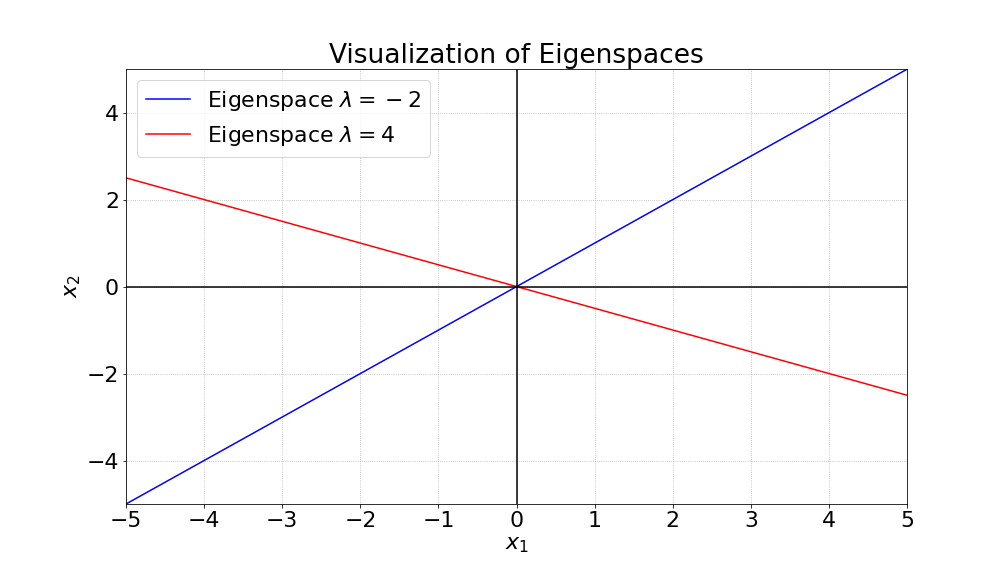
\includegraphics[width=2.5in]{images/fig-eigenspace2d.png}

  \column{0.5\tw}
  
  \pause
  Let $A = \begin{bmatrix} 2 & 0 & 0 \\ -1 & 3 & 1 \\ -1 & 1 & 3 \end{bmatrix}$. Find a basis for the eigenspace corresponding to the eigenvalue $\lambda = 2$.

  \[ \mathcal{B}_{\lambda =2} = \left\{ \begin{bmatrix} 1 \\ 1 \\ 0 \end{bmatrix} , \begin{bmatrix} 1 \\ 0 \\ 1 \end{bmatrix} \right\}. \]

  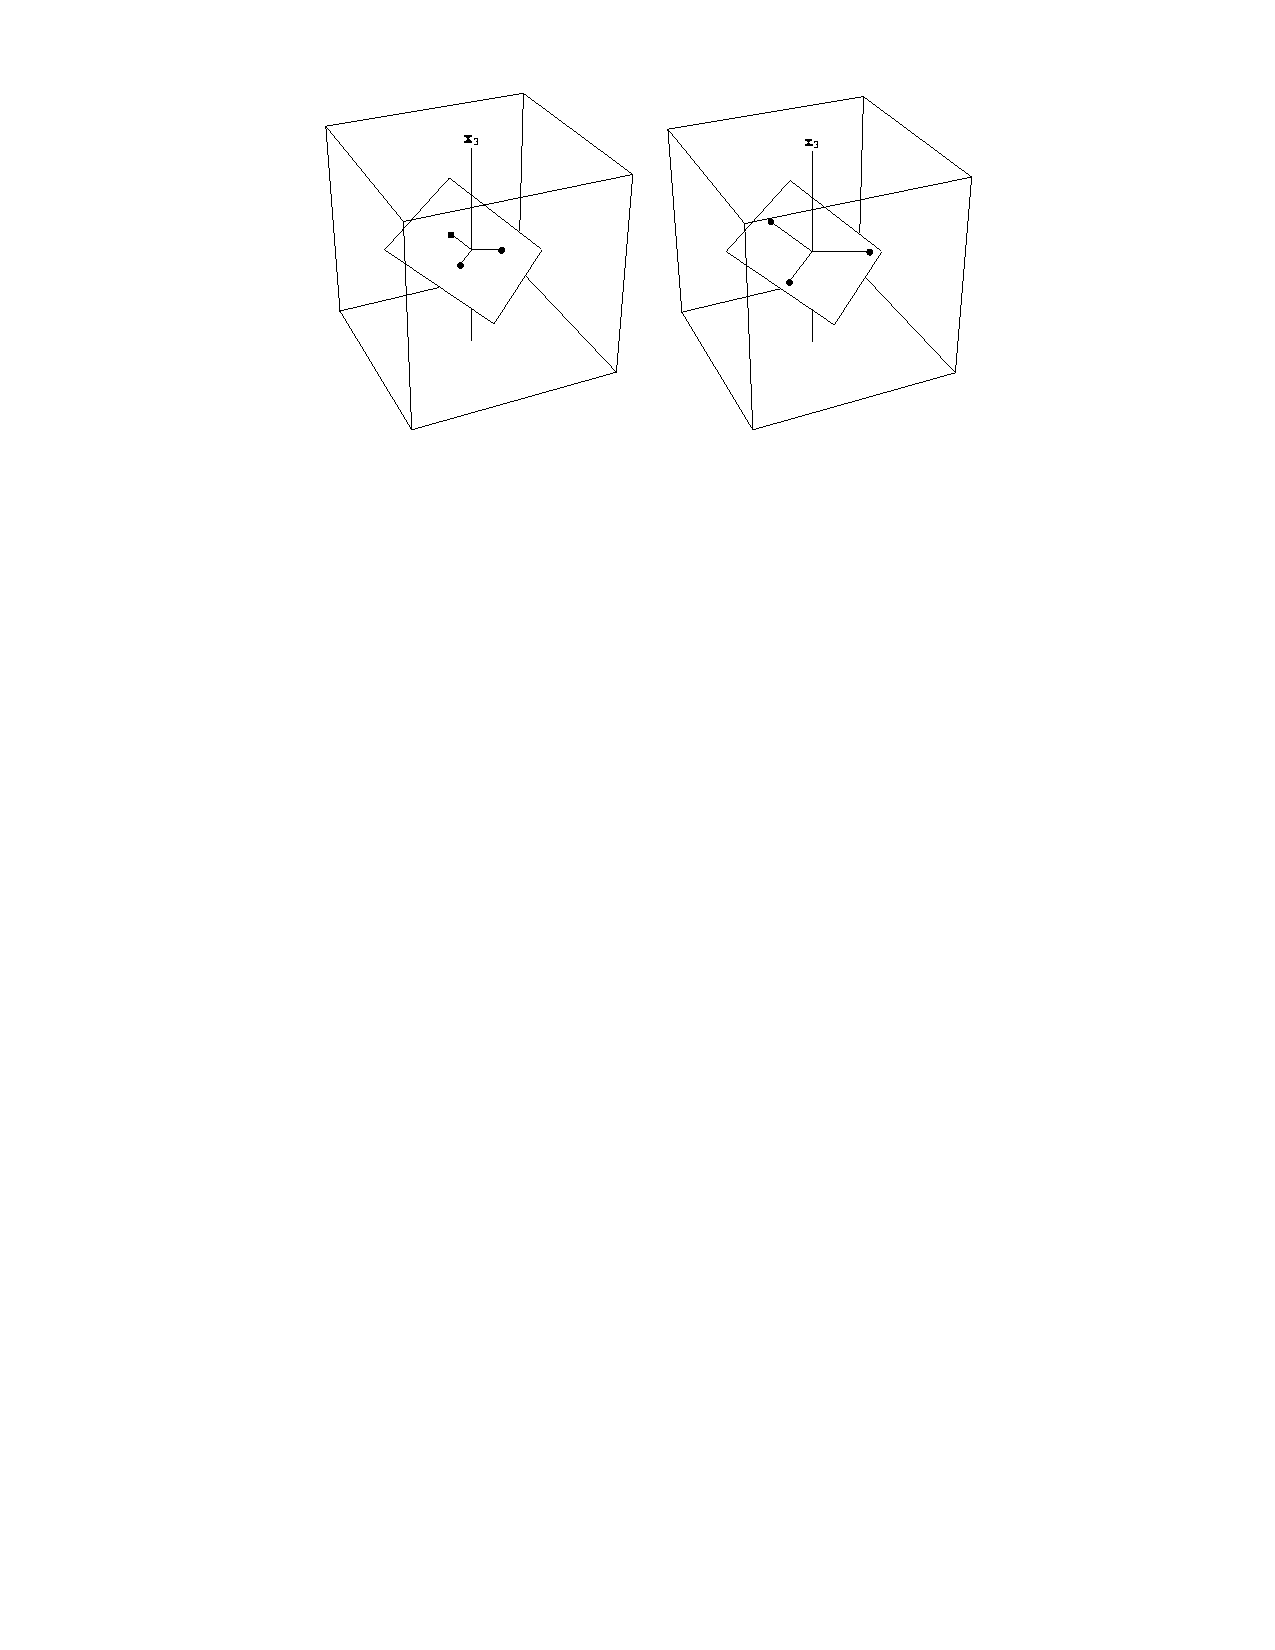
\includegraphics[width=2in]{images/fig-eigenspace3d.pdf}

  \end{columns}
\end{frame}


\begin{frame}{Finding Eigenvalues of $A^2$, $A^3$, $A^k$}
  \smallskip

  Let $A$ be an $n \times n$ matrix with eigenvalue $\lambda$ and corresponding eigenvector $\x$.

  \begin{enumerate}

  \item Show that $\lambda^2$ is an eigenvalue for $A^2$.
  \smallskip

  \pause
  \colorb{We have
  \[ A^2 \x = A (A \x) = A (\lambda \x ) = \lambda (A \x) = \lambda^2 \x. \]
  We see $\lambda^2$ is an eigenvalue of the matrix $A^2=AA$.}
  \bigskip

  \pause
  \item Show that $\lambda^3$ is an eigenvalue for $A^3$.
  \smallskip

  \alert{We have
  \[ A^3 \x = A (A^2 \x) = A (\lambda^2 \x ) = \lambda^2 (A \x) = \lambda^3 \x. \]
  We see $\lambda^3$ is an eigenvalue of the matrix $A^3$.}
  \end{enumerate}

  \pause
  \bbox
  In general, if $\lambda$ is an eigenvalue of $A$, then $\lambda^k$ is an eigenvalue of $A^k$, where $k$ is a positive integer.
  \ebox
\end{frame}


%\begin{frame}{Difference Equations}

%We can model some diseases with a \alert{difference equation} of the form

%\[ \begin{bmatrix} s_{k+1} \\ i_{k+1} \\ r_{k+1} \end{bmatrix} = A \begin{bmatrix} s_{k} \\ i_{k} \\ r_{k} \end{bmatrix} \]

%The simplest way to build a solution to the difference equation above is to find an eigenvector $\mathbf{x}_0 =  \begin{bmatrix} s_{0} \\ i_{0} \\ r_{0} \end{bmatrix}$ and its corresponding eigenvalue $\lambda$ and let

%\[ \mathbf{x}_k = \lambda^k \mathbf{x}_0 \quad \mbox{for } k = 1, 2, 3, \ldots .\] 

%This sequence is a solution since

%\[ A \mathbf{x}_k = A ( \lambda^k \mathbf{x}_0) = \lambda^k (A\mathbf{x_0}) = \lambda^{k+1} \mathbf{x_0} = \mathbf{x}_{k+1}.\]

%\end{frame}


%%%%%%%%%%%%%%%%%%%%%%%%%%%%%%%%%%%%%%%%%%%%%%%%%%%%%%%%%%%%%%%%%%%%%%%%%%%%%%%%%%%%%%%%%
\begin{frame}{Example 2}
  \medskip

  Is $5$ an \alert{eigenvalue} of $A = \begin{bmatrix} 6 & -3 & 1 \\ 3 & 0 & 5 \\ 2 & 2 & 6 \end{bmatrix}$?
  \bigskip

  \pause
  \[ (A - 5I) \mathbf{x} = \begin{bmatrix} 1 & -3 & 1 \\ 3 & -5 & 5 \\ 2 & 2 & 1 \end{bmatrix}  \mathbf{x} =  \begin{bmatrix} 0 \\ 0 \\0 \end{bmatrix} \]

  We have $\begin{bmatrix} 1 & -3 & 1 & 0 \\ 3 & -5 & 5 & 0 \\ 2 & 2 & 1 & 0 \end{bmatrix}
  \xrightarrow{\text{RREF}} \begin{bmatrix} 1 &  0 & 0 & 0 \\ 0 & 1 & 0 & 0 \\ 0 & 0 & 1 & 0 \end{bmatrix}$, 
  \pause
  which has only the \alert{trivial solution} $\x = \mathbf{0}$.
  \bigskip

  Since the equation $A\x=5\x$ has only the trivial solution, $\lambda =5$ is \alert{NOT} an eigenvalue of $A$.
\end{frame}


\begin{frame}{Eigenvalues of a Triangular Matrix}
  \begin{theorem}
  The eigenvalues of a \alert{triangular matrix} are the entries on its main diagonal.
  \end{theorem}
  \medskip

  \pause
  {\small
  \blue{Proof.}
  Let's consider the \alert{$3 \times 3$} case. Let $A$ be a $3 \times 3$ upper triangular matrix. Then
  \[ A - \lambda I = \begin{bmatrix} a_{11} & a_{12} & a_{13} \\ 0 & a_{22} & a_{23} \\ 0 & 0 & a_{33} \end{bmatrix} -
  \begin{bmatrix} \lambda & 0 & 0 \\ 0 & \lambda & 0 \\ 0 & 0 & \lambda \end{bmatrix} =
  \begin{bmatrix} a_{11}-\lambda & a_{12} & a_{13} \\ 0 & a_{22}-\lambda & a_{23} \\ 0 & 0 & a_{33}-\lambda \end{bmatrix}. \]

  The scalar $\lambda$ is an eigenvalue of $A$ if and only if there is a \blue{nontrivial solution} to the homogeneous equation $(A - \lambda I) \x = \mathbf{0}$.
  We have a nontrivial solution when $(A - \lambda I)$ has at least one \alert{free variable}.
  \pause
  \begin{itemize}
    \item If we set $\lambda=a_{11}$, then $x_1$ is free since there is no pivot in column 1.
    \item If we set $\lambda=a_{22}$, then $x_2$ is free since there is no pivot in column 2 (assuming that $\lambda\ne a_{11}$).
    \item If we set $\lambda=a_{33}$, then $x_3$ is free since there is no pivot in column 3 (assuming that $\lambda\ne a_{11},a_{22}$).
  \end{itemize}
  Thus the eigenvalues of $A$ are $\lambda = a_{11}$, $a_{22}$, or $a_{33}$.
  The argument follows similarly for larger matrices and for lower triangular matrices as well.
  \hfill\blue{\qed}
  } % small
\end{frame}


\begin{frame}{Linear Independence of Eigenvectors}
  %TODO: Should this be moved to the Diagonalization slides?  Seems rather random here.
  %\vspace*{-.5em}
  \begin{theorem}
  If $\v_1,\ldots,\v_p$ are eigenvectors corresponding to \colorr{distinct} eigenvalues $\lambda_1, \ldots, \lambda_p$ of an $n \times n$ matrix $A$, then the set $\left\{ \v_1, \ldots, \v_p \right\}$ is \colorr{linearly independent}.
  \end{theorem}
  %\vspace*{-1em}

  \pause
  {\small
  \blue{Proof.}
  Suppose $\left\{ \v_1, \ldots, \v_p \right\}$ is linearly dependent.
  Thus there are scalars $c_i$, not all zero, such that
  \vspace{-0.15in}
  \begin{equation}
  c_1 \v_1 + c_2 \v_2 + \ldots + c_p \v_p = \mathbf{0}.
  \end{equation}
  \vspace*{-0.3in}

  Among all such $c_i$s that are not all zero, choose the scalars such that the \colorb{fewest} $c_i$s are nonzero.
  Since the $v_i$s are eigenvectors and not the zero vector, at least two of the $c_i$s must be nonzero.  Assume that $c_j$ and $c_k$ are nonzero.

  \pause
  Multiplying both sides of equation (1) by $A$ gives
  \vspace{-0.15in}

  \begin{equation}
  A(c_1 \v_1 + \ldots +c_j \v_j + \ldots + c_p \v_p) = c_1 \lambda_1 \v_1 + \ldots +c_j \lambda_j \v_j + \ldots + c_p \lambda_p \v_p = \mathbf{0}.
  \end{equation}
  \vspace{-0.2in}

  \pause
  Multiplying both sides of equation (1) by $\lambda_j$ and subtracting from equation (2) gives
  \vspace{-0.15in}

  \begin{equation}
  c_1 (\lambda_1 - \lambda_j)\v_1 + c_2 (\lambda_2 - \lambda_j)\v_2 + \ldots + 0\v_j + \ldots + c_p (\lambda_p - \lambda_j)\v_p = \mathbf{0}.
  \end{equation}
  \vspace{-0.2in}

  \pause
  Note that $c_k (\lambda_k-\lambda_j)\ne 0$ since $\lambda_k\ne\lambda_j$.
  Thus, we have expressed $\mathbf{0}$ as a linear combination of $\v_1,\ldots,\v_p$ with not all scalars $0$ that has \colorb{fewer} zero scalars than what we assumed was the fewest. 
  \red{Contradiction!}
  \hfill\blue{\qed}
  }
\end{frame}

\end{document}


